\newpage
\drawBar{Introductie - Vervolg}
\noindent
\begin{minipage}[t]{.48\textwidth}
  \vspace{0.317cm}
  \zetKort{Zet - Hoger opleggen}{6_of_hearts}{7_of_hearts}{10_of_spades}{ace_of_spades2}{2_of_diamonds}{5_of_diamonds}{Hoger op een kaart met hetzelfde symbool.}
\end{minipage}% This must go next to `\end{minipage}`
\hspace{0.35cm} \vrule  \hspace{1.33cm}
\begin{minipage}[t]{.48\textwidth}
  \vspace{0.317cm}
  \zetKort{Zet - De aas en de 2}{ace_of_clubs}{2_of_clubs}{ace_of_hearts}{2_of_hearts}{ace_of_spades}{2_of_spades}{Een \kaart{2} op een \kaart{aas} met \ul{hetzelfde} symbool.}
\end{minipage}

\vspace{0.3cm}

\deelhoofdstuk{Zet - \'E\'entje lager opleggen en zelf drinken}
\noindent
\label{zetkort:offer_frits}
\vspace{-0.8cm}

\zetLang{2.5}{6_of_clubs}{5_of_clubs}{jack_of_diamonds}{10_of_diamonds}{\'E\'en lager op een kaart met hetzelfde symbool}{Proost op \quotes{offer Frits} en \textbf{neem een Fritsje}.}{}{}

\vspace{-0.0cm}

\vspace{0.5cm}
\deelhoofdstuk{Zetten - Andere spelers laten drinken}
\noindent
\label{sec:regels_kort}
\vspace{-0.8cm}

\def\localHeight{2.65}

\zetLang{2.64}{ace_of_hearts}{king_of_diamonds}{king_of_spades}{ace_of_hearts}{Een \kaart{koning} op een \kaart{harten aas}: \newline Een \kaart{harten aas} op een \kaart{koning}}{Andere spelers proosten op \quotes{kut Lisa} en \FritsenN.}{}{}

\vspace{-0.1cm}
\zetLang{\localHeight}{jack_of_clubs}{queen_of_hearts}{queen_of_diamonds}{jack_of_clubs}{Een \kaart{rode vrouw} op een \kaart{klaveren boer}: \newline Een \kaart{klaveren boer} op een \kaart{rode vrouw}}{Andere spelers proosten op \quotes{Chantal} en \FritsenN.}{}{}

\vspace{-0.1cm}
\zetLang{\localHeight}{queen_of_diamonds}{queen_of_clubs}{queen_of_spades}{queen_of_hearts}{Een \kaart{vrouw} op een \kaart{vrouw}}{Andere spelers proosten op \quotes{kut Kim} en \FritsenN.}{}{\ul{\texttt{LET OP}}: Als de \kaart{vrouw} op een stapel met daarop al tenminste drie achtereenvolgende \kaart{vrouwen} wordt gelegd, moeten de andere spelers \textbf{een dubbele Frits nemen}.}{}

\vspace{-0.1cm}
\zetLangMetKruis{\localHeight}{9_of_clubs}{9_of_diamonds}{black_joker}{9_of_spades}{Een \kaart{9} op een kaart ongelijk aan een \kaart{joker}}{}{}{\ul{\texttt{LET OP}}: Als de \kaart{9} op een \kaart{9} wordt gelegd, moeten de andere spelers proosten op \quotes{iedereen dubbelfrits} en \textbf{een dubbele Frits nemen}.}

\vspace{-0.1cm}
\zetLangMetKruis{\localHeight}{red_joker}{black_joker}{10_of_spades}{black_joker}{Een \kaart{joker} op de jokerstapel}{Begin een nieuwe jokerstapel als er nog geen jokerstapel ligt.}{Andere spelers proosten op \quotes{Frits} en \FritsenN.}{\ul{\texttt{LET OP}}: Niet gebruiken met \'e\'en kaart in je hand! \\ \ul{\texttt{LET OP}}: Er is maar \ul{\'e\'en} jokerstapel! \\ \ul{\texttt{LET OP}}: De jokerstapel bevindt zich direct naast de \ul{dichte} stapel!}

\vspace{0.58cm}
\centerline{\Large{\textbf{De volgende pagina bevat zetten voor ervaren spelers}}}

\newpage
\drawBar{Introductie - Vervolg}
\deelhoofdstuk{\proLabel Zet - De koning en aas tegelijkertijd}
\noindent
\vspace{-0.8cm}

\zetKoningAas{diamonds}{hearts}{spades}{clubs}{Een \kaart{koning} en een \kaart{aas} van hetzelfde symbool achterelkaar op een \kaart{vrouw} van hetzelfde symbool}

\vspace{-0.5cm}
\deelhoofdstuk{\proLabel Zet - Kaarten inwisselen}
\noindent
\label{zetkort:thierry}
\vspace{-0.8cm}

\zetLang{3.5}{queen_of_diamonds}{6_of_hearts}{queen_of_clubs}{6_of_diamonds}{Een \kaart{6} op een \kaart{vrouw}}{Proost op \quotes{Baudet} en \textbf{neem een dubbele Frits}.}{Geef je kaarten \textul{dicht} aan \FritsN. \Frits legt de kaarten onderop de dichte stapel en geeft je evenveel nieuwe kaarten.}{\ul{\texttt{LET OP}}: Niet gebruiken met \'e\'en kaart in je hand! \\ \ul{\texttt{LET OP}}: Iedereen kan het inwisselen blokkeren door meteen een \\ \kaart{klaveren 3} op de net opgelegde \kaart{6} te leggen!}

\deelhoofdstuk{\proLabel Zet - Andere spelers blokkeren}
\noindent
\label{zetkort:caroline}
\vspace{-0.8cm}

\zetLang{3.5}{jack_of_clubs}{6_of_diamonds}{jack_of_hearts}{6_of_spades}{Een \kaart{6} op een \kaart{boer}}{Proost op \quotes{van der Plas} en \textbf{neem een dubbele Frits}.}{(Ver)plaats het shotglaasje naar/op \'e\'en van de \ul{open} stapels.\\ Niemand mag nu opleggen op de stapel met het shotglaasje en de stapels die er direct orthogonaal aan grenzen.}{\ul{\texttt{LET OP}}: Niet gebruiken met \'e\'en kaart in je hand! \\ \ul{\texttt{LET OP}}: Haal het shotglaasje in je volgende beurt weer weg! \\ \ul{\texttt{LET OP}}: Iedereen kan het plaatsen blokkeren door meteen een \\ \kaart{klaveren 3} op de net opgelegde \kaart{6} te leggen!}

\vspace{1.2cm}

\noindent
\begin{minipage}[t]{.48\textwidth}
  \adjustbox{trim={0cm} {0.6cm} {0cm} {0.6cm},clip}%
  {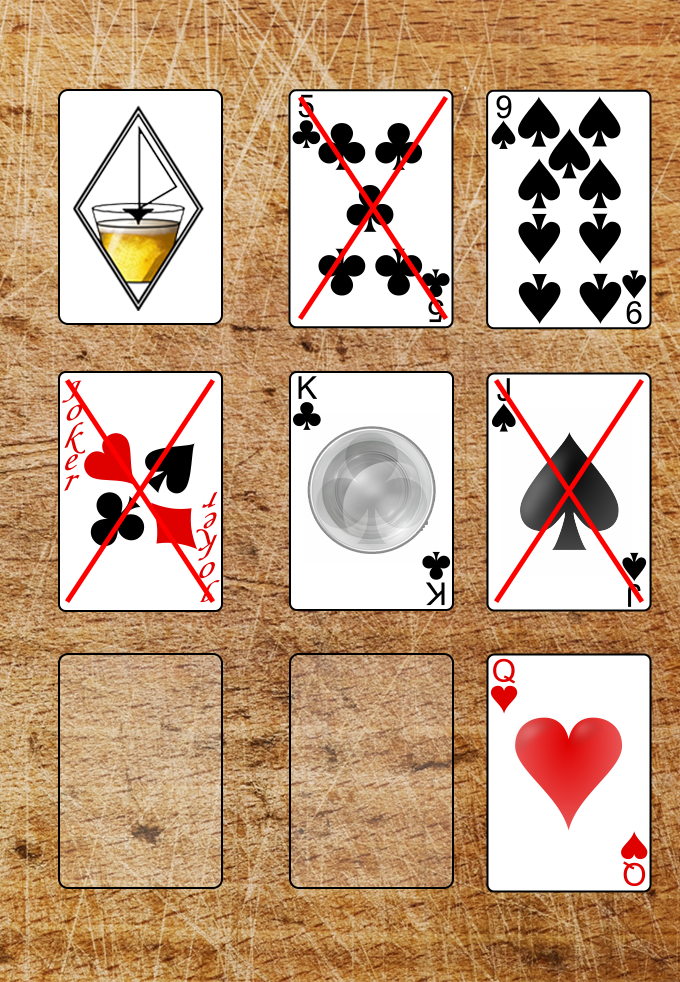
\includegraphics[,width=1\textwidth]{img/FritsPlank._Caroline1.png}}
\end{minipage}
\hfill \vrule  \hspace{0.20cm}
\begin{minipage}[t]{.48\textwidth}
  \adjustbox{trim={0cm} {0.6cm} {0cm} {0.6cm},clip}%
  {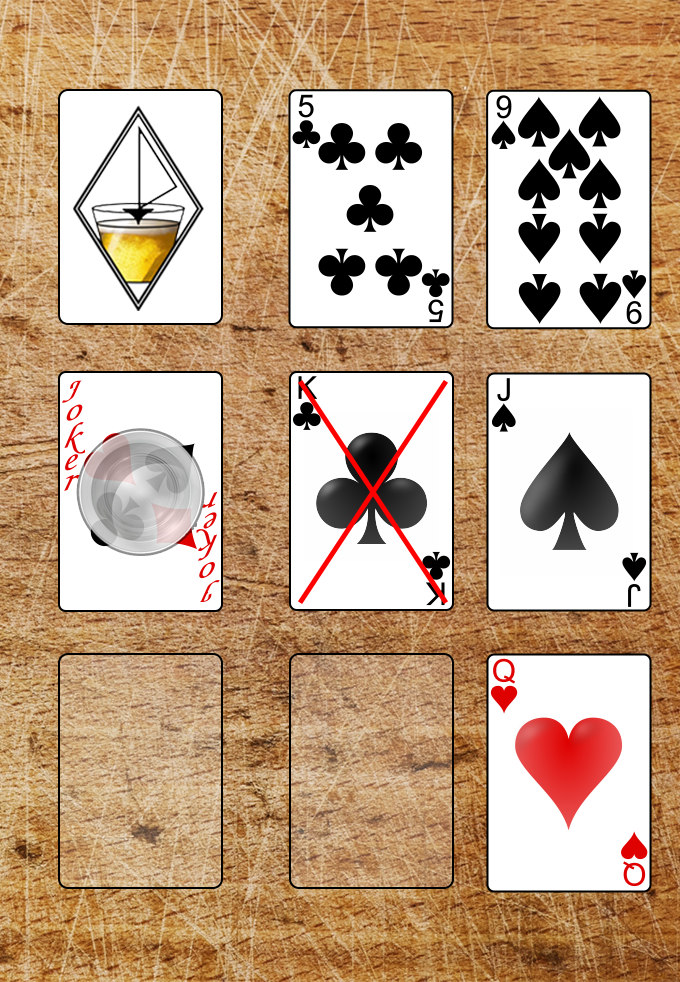
\includegraphics[width=1\textwidth]{img/FritsPlank._Caroline2.png}}
\end{minipage}

\vspace{0.5cm}

\centerline{\Large{\textbf{De rest van dit document beschrijft Fritsen in detail}}}